\chapter{Computerized Maintenance Management System (CMMS)}
\label{cmms}

Computerized Maintenance Management System ou em português Sistema Informatizado de Gestão de Manutenção, os CMMS, também conhecidos como Enterprise Asset Management (EAM) são softwares desehados para simplificar a gestão da manutenção.

Para melhor entender o que são essas ferramentas a MicroMain corporation quebrou o termo para explicar o uso de cada componente individualmente \cite{micromain}.

\textbf{Computerized}

Significa que com a ferramenta CMMS os dados sobre a manutenção estarão guardados em um computador. Hoje em dia esse conceito é muito comum, guardar dados no computador, mas antigamente, antes dos anos 1980, esses dados eram armazenados com o uso de papel e lápis, o que tornava a manutenção muito mais reativa do que proativa, ou seja, ela era realizada quando algo de errado acontecia. 

Nessa época era um pouco difícil pensar realizar manutenção preventiva, por existir a dificuldade de manter o tracking (rastro) de qual ativo precisaria de manutenção rotineira, quando todo o histórico deles era mantido em um sistema de arquivamento físico, em uma gaveta. 

Foi então que no final do anos 80 e começo dos anos 90, começou a surgir os CMMS, como solução para esses problemas, as organizações migraram seus dados sobre manutenção para seus computadores e começaram a ter a possibilidade de rastrear as ordens de serviço, gerar relatórios mais rápido e determinar quais ativos precisariam de manutenção preventiva. Ajundando a diminuir gastos e aumentar os lucros. 

\textbf{Maintenance}

Manutenção é a atividade realizada pelos usuários do CMMS todos os dias, seja por demanda, ordem de serviço ou inspeções de rotina. O software não substitui o trabalho humano, mas ele ajuda a determinar quais tarefas estão priorizadas adequadamente e que todo está em seu devido lugar (inventário, trabalho, etc). O software permite que o gestor e sua equipe foque mais no trabalho e menos na parte burocrática. 

\textbf{Manegement}

É a principal função do software, que foi desenhado para que os usuários possam saber sobre o estado da manutenção, com horários, ordens de serviço, previsões de inventário e acesso a relatórios de forma imediata. 

\textbf{System}

Sistema pode ser visto como a combinação geral de caracteríticas do CMMS, que variam de acordo com os diferenes tipos de CMMS.

Quando explicado os componente um a um, percebe-se qual a real função desse software, desenhado para facilitar e melhorar a forma como é realizada a Gestão da Manutenção. 

\section{Ferramenta Capterra}

A ferramenta Capterra, é um site onde encontram-se softwares voltados para diferentes tipos de negócio \cite{capterra}. Nela o usuário pesquisa sobre o software desejado e é devolvido uma série de resultados, que podem ser filtrados de acordo com a nessidade do usuário.

Por meio desta ferramenta foram encontrados diversos tipos de softwares CMMS, podendo consultar um tipo específico, por meio dos filtro, como mostra a Figura~\ref{filtro_capterra} e também ver o perfil do software escolhido que traz informações sobre o fornecedor Figura~\ref{informaca_capterra} e um checklist com as features do software Figura~\ref{checklist_capterra}, uma forma prática e simples de comparação de características existentes entre os diferentes tipos de CMMS disponíveis.

As imagens abaixo são exemplos de como são disponibilizadas as informções sobre um software no site Capterra.

\graphicspath{{figuras/}}
\begin{figure}[h]
\centering
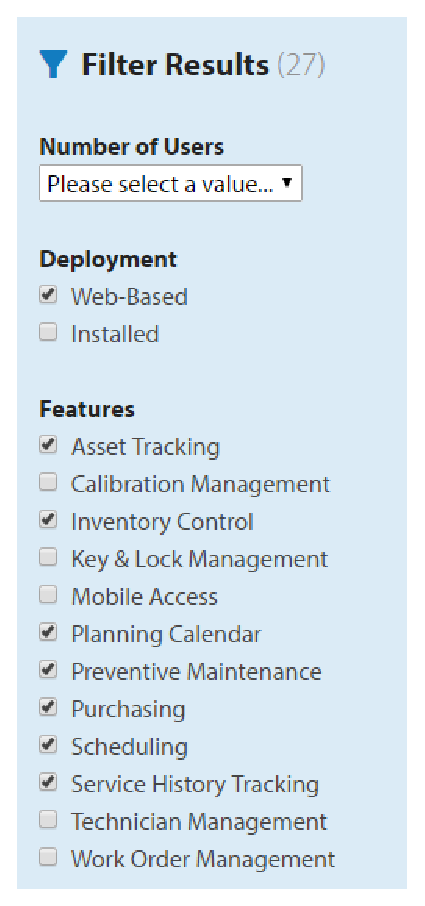
\includegraphics[width=0.5\textwidth]{filtro_capterra.eps}
\caption{Tipos de filtro do Capterra. \textbf{Fonte: http://www.capterra.com/cmms-software/.}}
\label{filtro_capterra}
\end{figure}


\graphicspath{{figuras/}}
\begin{figure}[h]
\centering
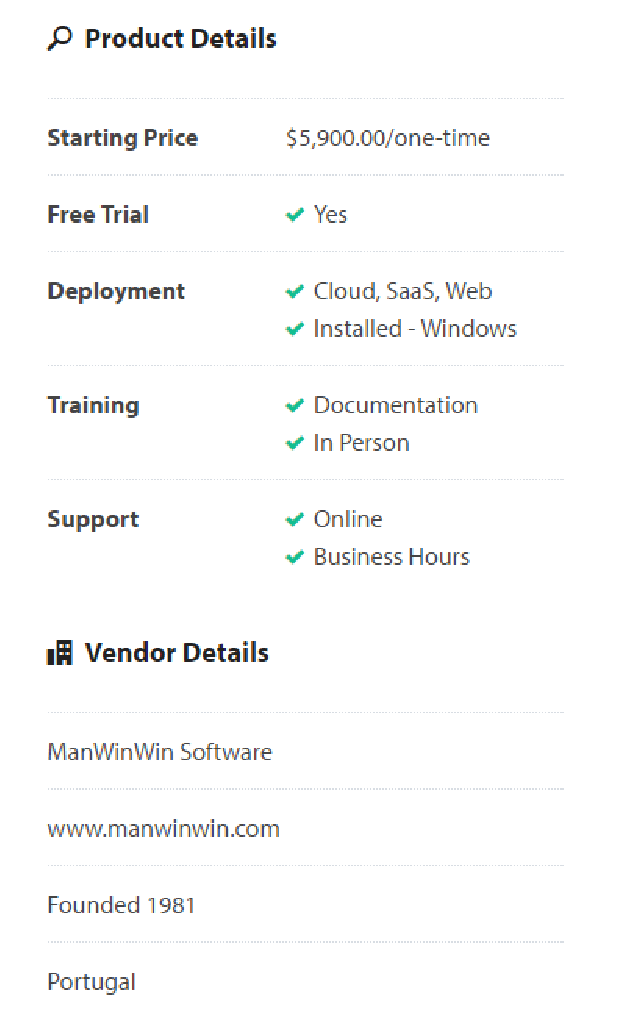
\includegraphics[width=0.5\textwidth]{informacao_capterra.eps}
\caption{Informações sobre o fornecedor do software ManWinWin. \textbf{Fonte: http://www.capterra.com/cmms-software/spotlight/109248/ManWinWin/ManWinWin\%20Software.}}
\label{informaca_capterra}
\end{figure}


\graphicspath{{figuras/}}
\begin{figure}[h]
\centering
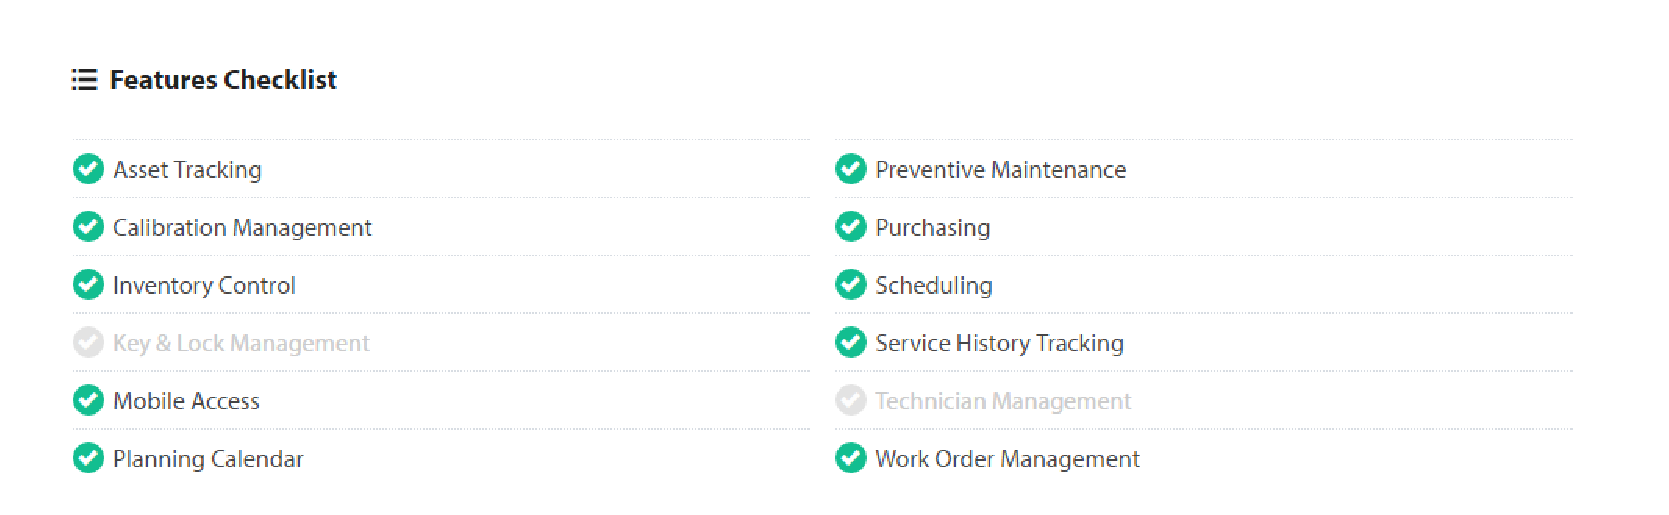
\includegraphics[width=0.9\textwidth]{checklist_capterra.eps}
\caption{Checklist com Features do software ManWinWin. \textbf{Fonte: http://www.capterra.com/cmms-software/spotlight/109248/ManWinWin/ManWinWin\%20Software.}}
\label{checklist_capterra}
\end{figure}

Com o uso desta ferramenta foi possível acessar diferentes CMMS e fazer uma tabela comparando suas caracterícas de acordo com o padrão do site \cite{capterra}, mostrado na Figura~\ref{checklist_capterra}. 

Na Figura~\ref{checklist_capterra} é mostrado o comparativo de algumas delas.

\graphicspath{{figuras/}}
\begin{figure}[h]
\centering
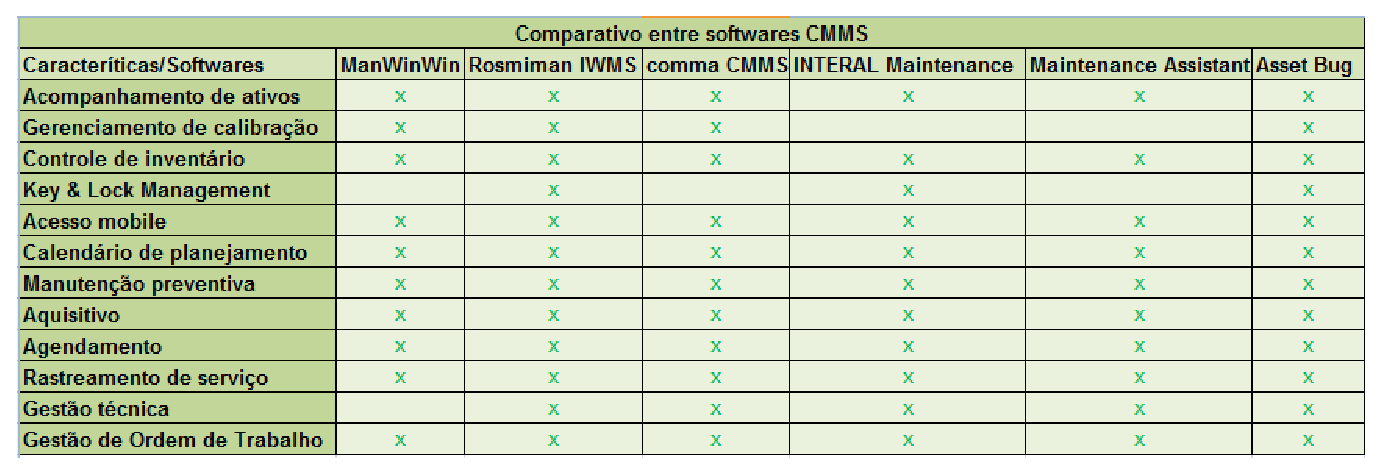
\includegraphics[width=1.0\textwidth]{feat_cmms.eps}
\caption{Comparativo entre caracteristicas dos softwares CMMS. \textbf{Fonte: http://www.capterra.com}}
\label{checklist_capterra}
\end{figure}

Por meio do conhecimento das principais características que esses softwares oferecem, foi constatado que a solução proposta no trabalho, será de grande valia quando informatizada, pois existem cáculos relativos a solução, geralmente gerados em uma ferramenta como o MATLAB, mas que não são integrados a um software como os CMMS. O que facilitaria o cotidiano do gestor e demais usuários, pois todas as informações necessária para suas avaliações e tomada de decisões poderão ser encontradas em um único sistema.